\section{Transformada Inversa}

\subsection{Introducción}

El método de Transformada Inversa es una de las tres técnicas vistas en la materia (junto con Rechazo y Composición) para generar valores de una variable aleatoria continua a partir de números aleatorios uniformes $0 < R < 1$. En este problema se aplica a una función $f(x)$ definida por tramos en el intervalo $[0,6]$.

\subsection{Descripción del problema}

La función proporcionada es:
\[
f(x)=\begin{cases}\dfrac{(x-3)^2}{18} &;\ 0 \leq x \leq 6 \\ 0 &;\ 0 > x > 6\end{cases}
\]

El objetivo consiste en generar valores aleatorios mediante el método de transformada inversa y verificar que los valores obtenidos pertenezcan al intervalo $[0,6]$.

Representación gráfica:

\begingroup
\tracinglostchars=0
\begin{figure}[H]
\centering
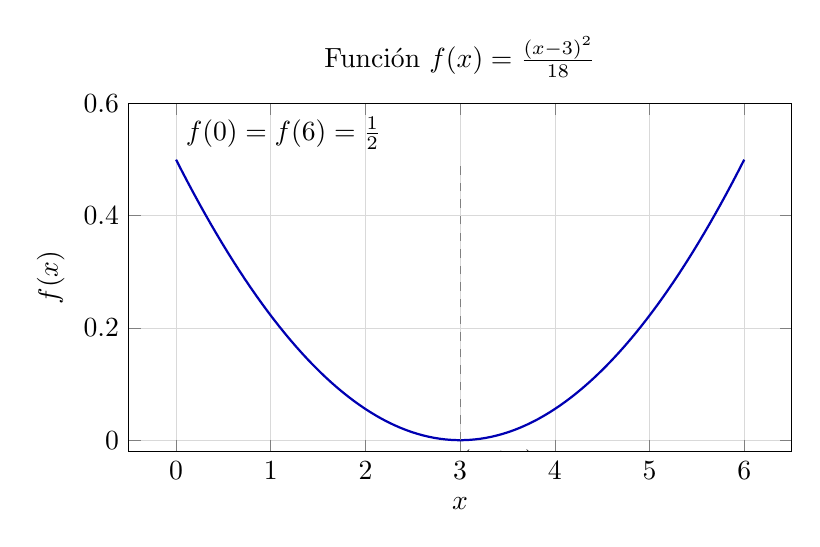
\begin{tikzpicture}
\begin{axis}[
  width=10cm, height=6cm,
  xlabel={$x$}, ylabel={$f(x)$},
  xmin=-0.5, xmax=6.5,
  ymin=-0.02, ymax=0.6,
  grid=both, grid style={line width=0.2pt, draw=gray!30},
  title={Función $f(x) = \frac{(x-3)^2}{18}$},
  xtick={0,1,2,3,4,5,6},
  samples=100
]
\addplot[blue!70!black, thick, domain=0:6] {(x-3)^2/18};
\addplot[dashed, gray] coordinates {(3,0) (3,0.5)};
\node[below] at (axis cs:3,0) {$x=3$ (mín.)};
\node[above right] at (axis cs:0,0.5) {$f(0)=f(6)=\frac{1}{2}$};
\end{axis}
\end{tikzpicture}
\caption{Gráfica de la función proporcionada. Nótese que el mínimo se alcanza en $x=3$ y los valores máximos en los extremos $x=0$ y $x=6$.}
\end{figure}
\endgroup

\subsection{Propuesta de solución}

Se aplica el método de Transformada Inversa, que requiere seguir los siguientes cinco pasos:

\textbf{Paso 1: Contar con la función $f(x)$}

Sea $f(x)$:
\[
f(x)=\begin{cases}\dfrac{(x-3)^2}{18} &;\ 0 \leq x \leq 6 \\ 0 &;\ 0 > x > 6\end{cases}
\]

\textbf{Paso 2: Determinar la función acumulada}

Calculamos la función de distribución acumulada $F(x)$ integrando $f(x)$:
\[F(x) = \int_0^x \frac{(x-3)^2}{18}\, dx\]

Desarrollo:
\begin{align*}
F(x) &= \frac{1}{18} \int_0^x (x-3)^2\, dx \\[4pt]
     &= \frac{1}{18} \left[\frac{(x-3)^3}{3}\right]_0^x \\[4pt]
     &= \frac{1}{18} \left(\frac{(x-3)^3}{3} - \frac{(0-3)^3}{3}\right) \\[4pt]
     &= \frac{1}{18} \left(\frac{(x-3)^3}{3} + \frac{27}{3}\right) \\[4pt]
     &= \frac{1}{18} \cdot \frac{(x-3)^3 + 27}{3}
\end{align*}

\[
\boxed{F(x) = \frac{(x-3)^3 + 27}{54}}, \quad 0 \leq x \leq 6
\]

\textbf{Paso 3: Igualar la función acumulada}

Igualamos la función acumulada $F(x)$ con un número aleatorio $R$:
\[F(x) = R\]

Sustituyendo la expresión de $F(x)$:
\[\frac{(x-3)^3 + 27}{54} = R\]

\textbf{Paso 4: Aplicar función inversa}

Despejamos $x = F^{-1}(R)$ de la ecuación anterior:

\begin{align*}
\frac{(x-3)^3 + 27}{54} &= R \\[4pt]
(x-3)^3 + 27 &= 54R \\[4pt]
(x-3)^3 &= 54R - 27 \\[4pt]
x - 3 &= \sqrt[3]{54R - 27} \\[4pt]
x &= 3 + \sqrt[3]{54R - 27}
\end{align*}

\[
x=\begin{cases}3+\sqrt[3]{54R-27} &;\ 0 \leq R \leq 1 \\ 0 &;\ 0 > R > 1\end{cases}
\]

\subsection{Objetivos}

\textbf{Objetivo general:} Aplicar el método de Transformada Inversa para generar valores aleatorios de la variable $x$ con función de densidad $f(x)=\dfrac{(x-3)^2}{18}$.

\textbf{Objetivos específicos:}
\begin{enumerate}
    \item Obtener la función inversa $x = F^{-1}(R)$ a partir de la función acumulada $F(x)$.
    \item Validar mediante prueba de escritorio que los valores generados pertenecen al intervalo $[0,6]$.
\end{enumerate}

\subsection{Desarrollo de la solución}

\subsubsection{Algoritmo}

Del modelamiento se obtiene la propuesta algorítmica para generar la variable aleatoria $x$:

\begin{lstlisting}[caption={Algoritmo — Generación de variable aleatoria}, language=Pascal]
real funcion variableTransformadaInversa(real R){
    real x;
    x <- 3 + RaizCubica(54*R - 27);
    retornar x;
}
\end{lstlisting}

La función recibe un número aleatorio $0 < R < 1$ y retorna $x$ aplicando directamente la transformada inversa $x = 3 + \sqrt[3]{54R - 27}$ obtenida en el Paso 4 de la propuesta de solución.

\subsubsection{Diagrama de flujo}

\begin{figure}[H]
\centering
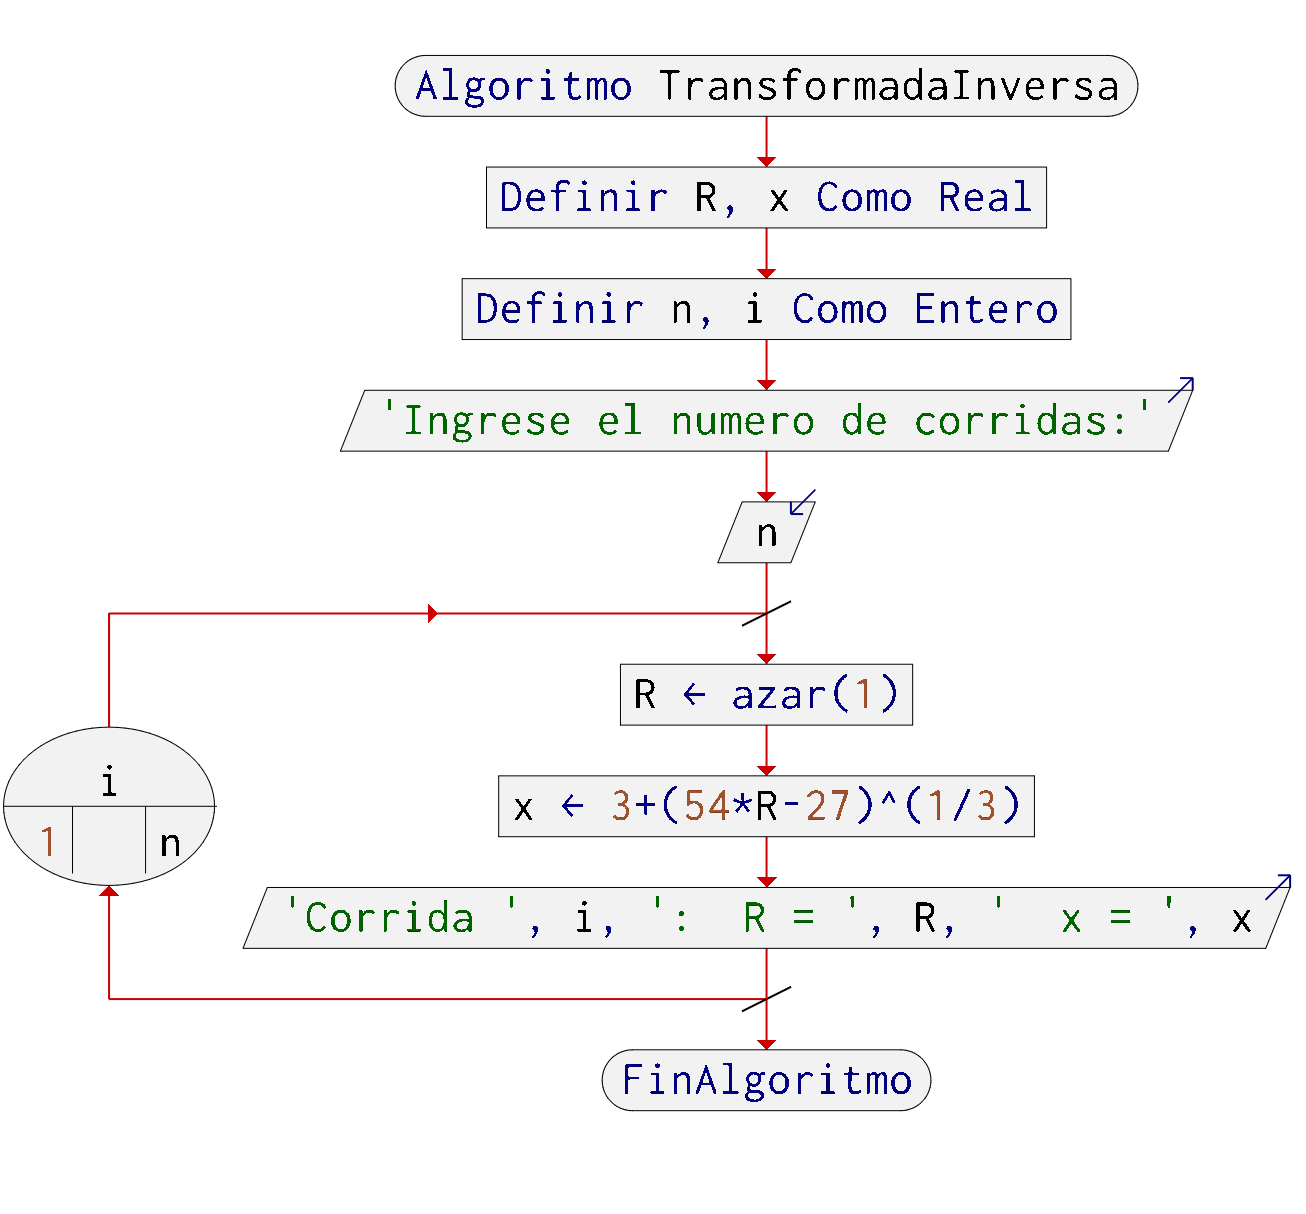
\includegraphics[width=0.8\textwidth]{capturas_pseint/p1_transformada_inversa.png}
\caption{Diagrama de flujo — Transformada Inversa (PSeInt)}
\end{figure}

\subsubsection{Tabla de simulación}

Cada fila es una corrida; cada columna es un paso del algoritmo:

\begin{mitabla}[H]{Tabla de simulación con $n=10$}
\begin{tabular}{c cc}
\toprule
Corrida & $R \leftarrow \text{gcm}()$ & $x = 3+\sqrt[3]{54R-27}$ \\
\midrule
1  & 0,9709 & $3+\sqrt[3]{54(0{,}9709)-27} = 5{,}9406$ \\
2  & 0,6970 & $3+\sqrt[3]{54(0{,}6970)-27} = 5{,}1994$ \\
3  & 0,3014 & $3+\sqrt[3]{54(0{,}3014)-27} = 0{,}7947$ \\
4  & 0,9728 & $3+\sqrt[3]{54(0{,}9728)-27} = 5{,}9445$ \\
5  & 0,8182 & $3+\sqrt[3]{54(0{,}8182)-27} = 5{,}5806$ \\
6  & 0,4939 & $3+\sqrt[3]{54(0{,}4939)-27} = 3{,}9563$ \\
7  & 0,7423 & $3+\sqrt[3]{54(0{,}7423)-27} = 5{,}2956$ \\
8  & 0,1593 & $3+\sqrt[3]{54(0{,}1593)-27} = 1{,}4297$ \\
9  & 0,0821 & $3+\sqrt[3]{54(0{,}0821)-27} = 0{,}6372$ \\
10 & 0,5821 & $3+\sqrt[3]{54(0{,}5821)-27} = 4{,}6902$ \\
\bottomrule
\end{tabular}
\end{mitabla}

\subsubsection{Implementación}

\begin{mitabla}[H]{Variables del modelamiento}
\begin{tabular}{cL{8cm}c}
\toprule
Variable & Descripción & Paso \\
\midrule
$R$ & Número aleatorio uniforme $0 < R < 1$, generado con \texttt{random()} & Paso 3 \\
$x$ & Variable aleatoria: $x = 3 + \sqrt[3]{54R - 27}$ & Paso 4 \\
\bottomrule
\end{tabular}
\end{mitabla}

\textbf{Implementación en Java:}

\begin{lstlisting}[caption={TransformadaInversa.java}, language=Java]
import java.util.Scanner;

public class TransformadaInversa {

    public static double generarX() {
        double R = Math.random();
        double x = 3 + Math.cbrt(54 * R - 27);
        return x;
    }

    public static void main(String[] args) {
        Scanner sc = new Scanner(System.in);
        System.out.print("Ingrese el numero de corridas n: ");
        int n = sc.nextInt();

        System.out.println("\nCorrida\tR\t\tx");
        for (int i = 1; i <= n; i++) {
            double R = Math.random();
            double x = 3 + Math.cbrt(54 * R - 27);
            System.out.printf("%d\t%.4f\t\t%.4f%n", i, R, x);
        }
        sc.close();
    }
}
\end{lstlisting}

\textbf{Implementación en Excel:}

\begin{figure}[H]
\centering
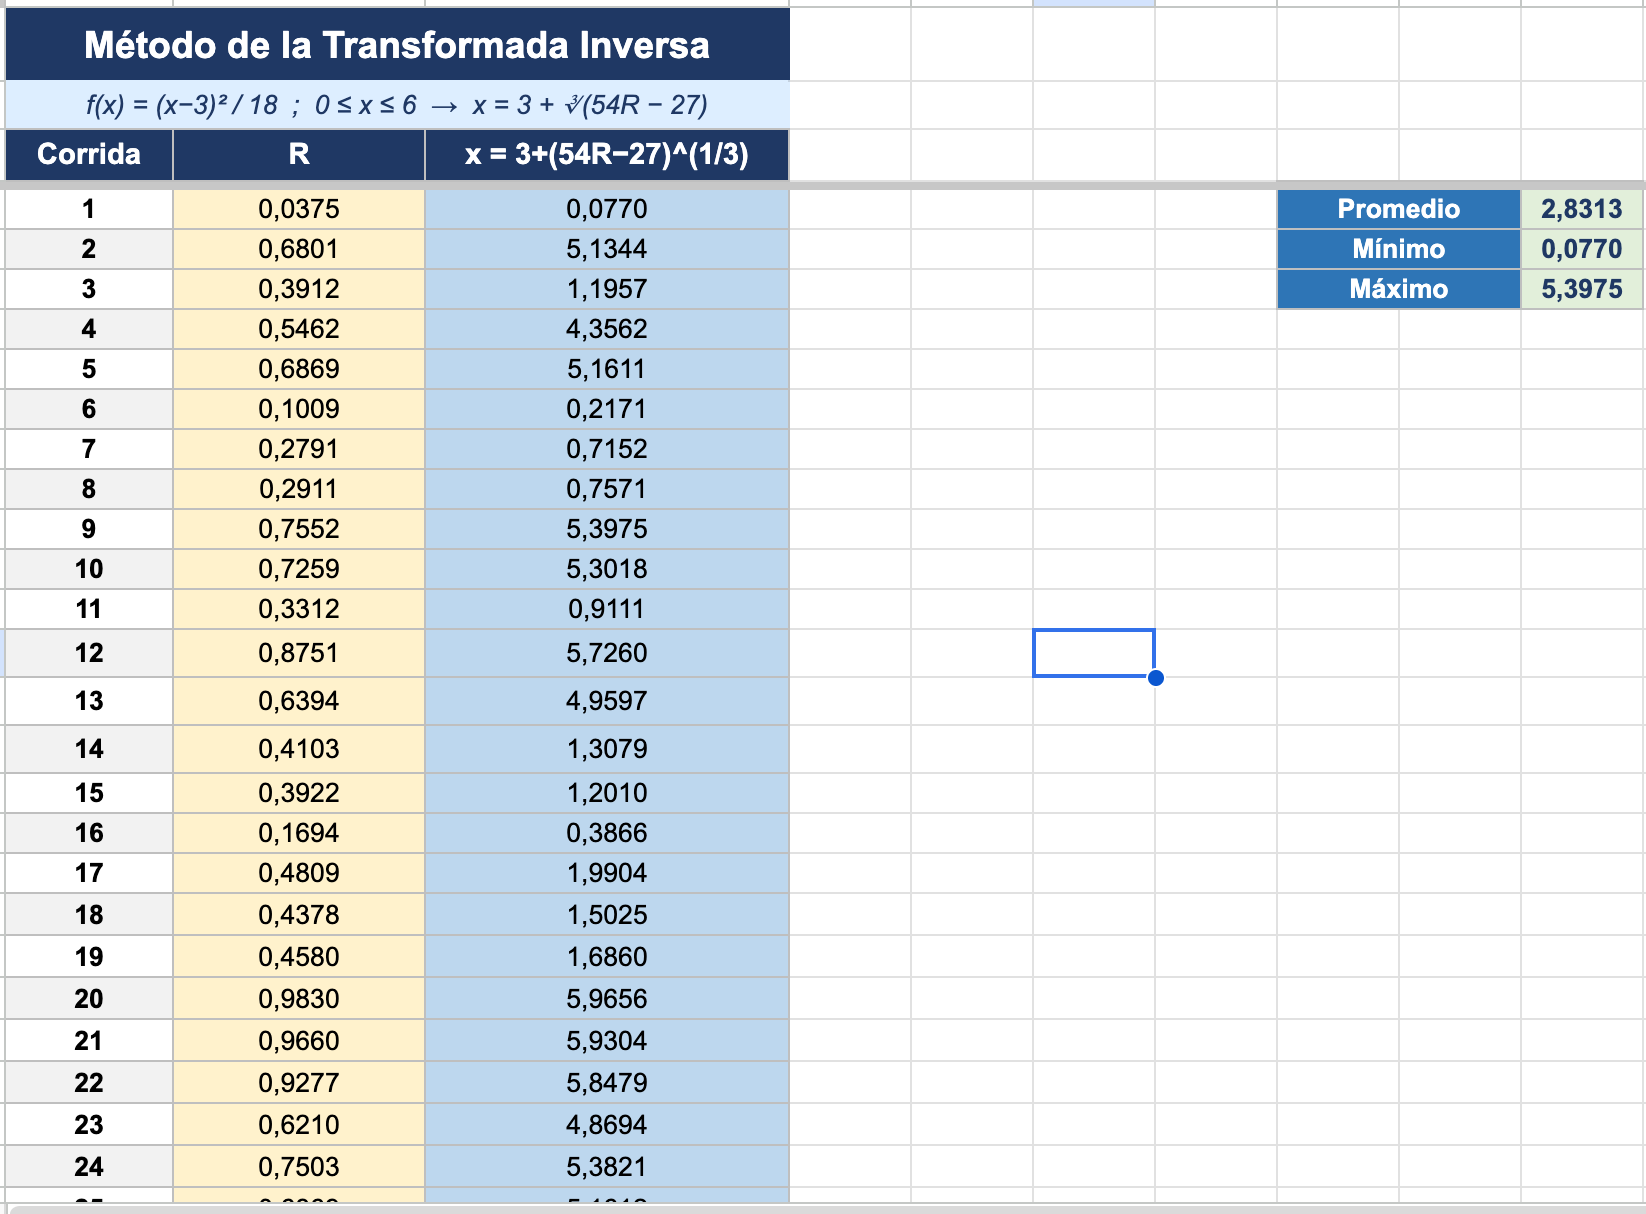
\includegraphics[width=0.9\textwidth]{capturas_excel/p1_transformada_inversa.png}
\caption{Hoja de cálculo — Transformada Inversa}
\end{figure}

\subsection{Validación}

\subsubsection{\texorpdfstring{Prueba de escritorio con $n=25$}{Prueba de escritorio con n=25}}

\begin{mitabla}[H]{\texorpdfstring{Validación con $n=25$ corridas}{Validacion con n=25 corridas}}
\begin{tabular}{ccc}
\toprule
Corrida & $R$ & $x=3+\sqrt[3]{54R-27}$ \\
\midrule
1 & 0,9663 & $3+\sqrt[3]{54(0,9663)-27} = 5,9311$ \\
2 & 0,3438 & $3+\sqrt[3]{54(0,3438)-27} = 0,9644$ \\
3 & 0,3865 & $3+\sqrt[3]{54(0,3865)-27} = 1,1702$ \\
4 & 0,8691 & $3+\sqrt[3]{54(0,8691)-27} = 5,7112$ \\
5 & 0,6990 & $3+\sqrt[3]{54(0,6990)-27} = 5,2067$ \\
6 & 0,9047 & $3+\sqrt[3]{54(0,9047)-27} = 5,7958$ \\
7 & 0,5043 & $3+\sqrt[3]{54(0,5043)-27} = 3,6150$ \\
8 & 0,8624 & $3+\sqrt[3]{54(0,8624)-27} = 5,6948$ \\
9 & 0,1001 & $3+\sqrt[3]{54(0,1001)-27} = 0,2153$ \\
10 & 0,8215 & $3+\sqrt[3]{54(0,8215)-27} = 5,5894$ \\
11 & 0,5857 & $3+\sqrt[3]{54(0,5857)-27} = 4,6667$ \\
12 & 0,6718 & $3+\sqrt[3]{54(0,6718)-27} = 5,1012$ \\
13 & 0,9590 & $3+\sqrt[3]{54(0,9590)-27} = 5,9157$ \\
14 & 0,4151 & $3+\sqrt[3]{54(0,4151)-27} = 1,3387$ \\
15 & 0,3255 & $3+\sqrt[3]{54(0,3255)-27} = 0,8878$ \\
16 & 0,1749 & $3+\sqrt[3]{54(0,1749)-27} = 0,4010$ \\
17 & 0,8745 & $3+\sqrt[3]{54(0,8745)-27} = 5,7245$ \\
18 & 0,1367 & $3+\sqrt[3]{54(0,1367)-27} = 0,3030$ \\
19 & 0,6410 & $3+\sqrt[3]{54(0,6410)-27} = 4,9674$ \\
20 & 0,7793 & $3+\sqrt[3]{54(0,7793)-27} = 5,4706$ \\
21 & 0,0548 & $3+\sqrt[3]{54(0,0548)-27} = 0,1138$ \\
22 & 0,2243 & $3+\sqrt[3]{54(0,2243)-27} = 0,5401$ \\
23 & 0,1344 & $3+\sqrt[3]{54(0,1344)-27} = 0,2974$ \\
24 & 0,7730 & $3+\sqrt[3]{54(0,7730)-27} = 5,4520$ \\
25 & 0,8552 & $3+\sqrt[3]{54(0,8552)-27} = 5,6769$ \\
\bottomrule
\end{tabular}
\end{mitabla}

\subsubsection{\texorpdfstring{Corridas con $n \geq 50$}{Corridas con n mayor igual 50}}

Para validar el comportamiento del algoritmo con muestras más grandes, se ejecutaron corridas con $n = 50$, $100$, $250$, $500$, $1000$. Se muestra el último valor generado en cada corrida:

\begin{mitabla}{\texorpdfstring{Resumen de corridas con $n \geq 50$}{Resumen de corridas con n mayor igual 50}}
\begin{tabular}{ccc}
\toprule
$n$ & $R$ (última corrida) & $x=3+\sqrt[3]{54R-27}$ \\
\midrule
50 & 0,7999 & $3+\sqrt[3]{54(0,7999)-27} = 4,3196$ \\
100 & 0,1036 & $3+\sqrt[3]{54(0,1036)-27} = 0,5612$ \\
250 & 0,0323 & $3+\sqrt[3]{54(0,0323)-27} = 0,1749$ \\
500 & 0,1626 & $3+\sqrt[3]{54(0,1626)-27} = 0,8788$ \\
1000 & 0,0629 & $3+\sqrt[3]{54(0,0629)-27} = 0,3430$ \\
\bottomrule
\end{tabular}
\end{mitabla}

\subsection{Interpretación}

\subsubsection{Resultados}

En las 25 corridas de la prueba de escritorio, todos los valores de $x$ generados quedaron dentro del intervalo $[0,6]$ esperado, con valores más frecuentes hacia los extremos del intervalo y menor densidad cerca de $x=3$, lo cual es consistente con la forma de $f(x)$ (mínimo en $x=3$, máximos en $x=0$ y $x=6$). Las corridas con $n \geq 50$ mantienen el mismo comportamiento al aumentar el tamaño de muestra.

\subsubsection{Interpretación}

Los resultados confirman que la función inversa $x = 3 + \sqrt[3]{54R-27}$ obtenida en la propuesta de solución genera correctamente valores de la variable aleatoria $x$ según la densidad $f(x) = \frac{(x-3)^2}{18}$: ningún valor generado cae fuera de $[0,6]$, y la mayor concentración de valores en los extremos coincide con las zonas de mayor densidad de la función.

\subsection{Conclusión}

El método de Transformada Inversa permitió obtener una función cerrada $x=F^{-1}(R)$ a partir de la función de densidad dada, la cual se validó mediante prueba de escritorio (n=25 y $n \geq 50$) y se implementó tanto en Java como en Excel, obteniendo en ambos casos resultados consistentes con el modelo teórico.
